%%%%%%%%%%%%%%%%%%%%%%%%%%%%%%%%%%%%%%%%%%%%%%%%%%%%%%%%%%%%%%%%%
%
% Project     : Bachelorarbeit
% Title       : Machbarkeitsanalyse für eine ressourcenorientierte Schnittstelle zur Verarbeitung grundlegender Probleme der Informatik
% File        : projektplanung.tex Rev. 01
% Date        : 01.03.2015
% Author      : Raffael Santschi
%
%%%%%%%%%%%%%%%%%%%%%%%%%%%%%%%%%%%%%%%%%%%%%%%%%%%%%%%%%%%%%%%%%

\chapter{Projektplanung}\label{chap.projektplanung}
Dieses Kapitel handelt von der Projektplanung und den verschiedenen Arbeitspaketen für dieses Projekt.

\section{Meilensteine}\label{meilensteine}
Folgende Meilensteine wurden für dieses Projekt festgelegt:

\begin{table}[ht]
\centering
  \begin{tabular}{ l | r }
	\hline
	\rowcolor{gray}
	\textbf{Projektstart}			&	\textbf{23.01.2015}\\ \hline
	Anforderungsdokument fertig		&	28.02.2015	\\ \hline
	Wissen über Probleme aufgebaut		&	19.04.2015	\\ \hline
	Erster \gls{vertikaler_durchstich}		& 	26.04.2015	\\ \hline
	Architektur festgelegt			&	03.05.2015	\\ \hline
	Prototyp fertig				&	29.05.2015	\\ \hline
	Dokumentation fertig			&	12.06.2015	\\ \hline
	Dokumentation korrigiert			&	26.06.2015	\\ \hline
	Präsentation					&	08.07.2015 \\ \hline
  \end{tabular}
   \caption{Meilensteine}\label{table:milestones}
\end{table}

\section{Arbeitspakete}\label{arbeitspakete}
Das Projekt beinhaltet sieben Arbeitspakete:
\begin{itemize}
\item Planung
\item Analyse und Auswahl der Probleme
\item Requirement Engineering
\item Konzept
\item Umsetzung Prototyp
\item Testing
\item Dokumentation
\end{itemize}

\subsection{Planung}\label{planung}
In der Planungsphase wird geschaut, was in dem Projekt erreicht werden muss und wie diese Tätigkeiten auf die vorhandene Zeit aufgeteilt werden. Es wird auch das erste Mal mit dem 
\gls{stakeholder} geredet und erste Abmachungen getroffen.

\subsection{Analyse und Auswahl der Probleme}\label{analyse_auswahl_probleme}
Ein sehr wichtiges Paket ist die Analyse und die Auswahl der Probleme. Es ist wichtig, dass die Probleme möglichst vielfältig gewählt werden und sie gut analysiert werden, damit das Konzept 
mit den erhobenen Daten sauber geplant werden kann.

\subsection{Requirement Engineering}\label{rqe}
Bei der Erstellung eines neuen Systems ist es immer wichtig, dass die Grundanforderungen bekannt sind. Um die Anforderungen zu erfassen, wird der \gls{stakeholder} befragt, was seine Wünsche 
sind. Oft werden bei der Anforderungsanalyse einige Anforderungen nicht aufgelistet, sondern einfach vorausgesetzt, sogenannte \glspl{basisfaktor}. Diese Anforderungen müssen dann vom 
Entwickler erfasst werden. Der Anforderungskatalog wird nach der Vollendung nochmals mit dem \gls{stakeholder} in einem Review angeschaut (siehe dazu auch \cite{req_eng_book}).

\subsection{Konzept}\label{ref_backend}
Das Hauptziel dieser Arbeit ist ein Konzept, welches generisch ist und viele verschiedene Probleme mit wenig Aufwand verarbeiten kann. Die Architektur muss gut durchdacht sein und die 
Möglichkeiten müssen gegeneinander abgewägt werden. Schliesslich muss eine Konzept entstehen, welches in einem Prototypen umsetzbar ist.

\subsection{Umsetzung Prototyp}\label{eng_prototyp}
In diesem Arbeitspaket werden die Anforderungen mit dem festgelegten Konzept umgesetzt. Die Schnittstelle wird entworfen, die ersten Tests werden durchgeführt und Unstimmigkeiten in den 
Anforderungen werden mit dem \gls{stakeholder} geklärt.

\subsection{Testing}\label{testing}
Das Projekt benötigt automatische Tests, welche erstellt und überprüft werden müssen. Die Tests sollten einen Grossteil des Projekts abdecken und bei einer Anpassung oder Erweiterung des 
Codes Sicherheit bieten.

\subsection{Dokumentation}\label{dokumentation}
Die Dokumentation wird während des ganzen Projekts hindurch aktuell gehalten. Für das Erfassen dieses Dokuments wird \LaTeX\ und das \LaTeX-Template der ZHAW \cite{zhaw_latex_template} mit ein 
paar kleinen Anpassungen verwendet.

\section{Zeitplan}\label{zeitplan}
Der Zeitplan gibt eine grobe Übersicht, wann an dem Projekt gearbeitet werden kann und wann die verschiedenen Tätigkeiten fertig sein sollten. Die Angaben sind nur Richtwerte, da neben dem 
Projekt noch berufliche Verpflichtungen und andere Tätigkeiten Zeit benötigen.

\subsection{Geplante Abwesenheiten}
\begin{table}[ht]
\centering
  \begin{tabular}{ l | r }
	\hline
	\rowcolor{gray}
	\textbf{Abwesenheit}					&	\textbf{Start - Ende}	\\ \hline
	Ferien								&	07.02.2015 - 15.02.2015	\\ \hline
	Seminararbeiten						&	06.04.2015 - 19.04.2015	\\ \hline
	Modulprüfungen und Vorträge Seminararbeit		&	15.06.2015 - 28.06.2015	\\ \hline
  \end{tabular}
   \caption{Geplante Abwesenheiten}\label{table:holidays}
\end{table}

\newpage 

\subsection{Projektplan}\label{projektplan}
Der Zeitplan basierend auf den Arbeitspaketen und den geplanten Abwesenheiten sieht wie folgt aus:
\begin{figure}[h]
\centering
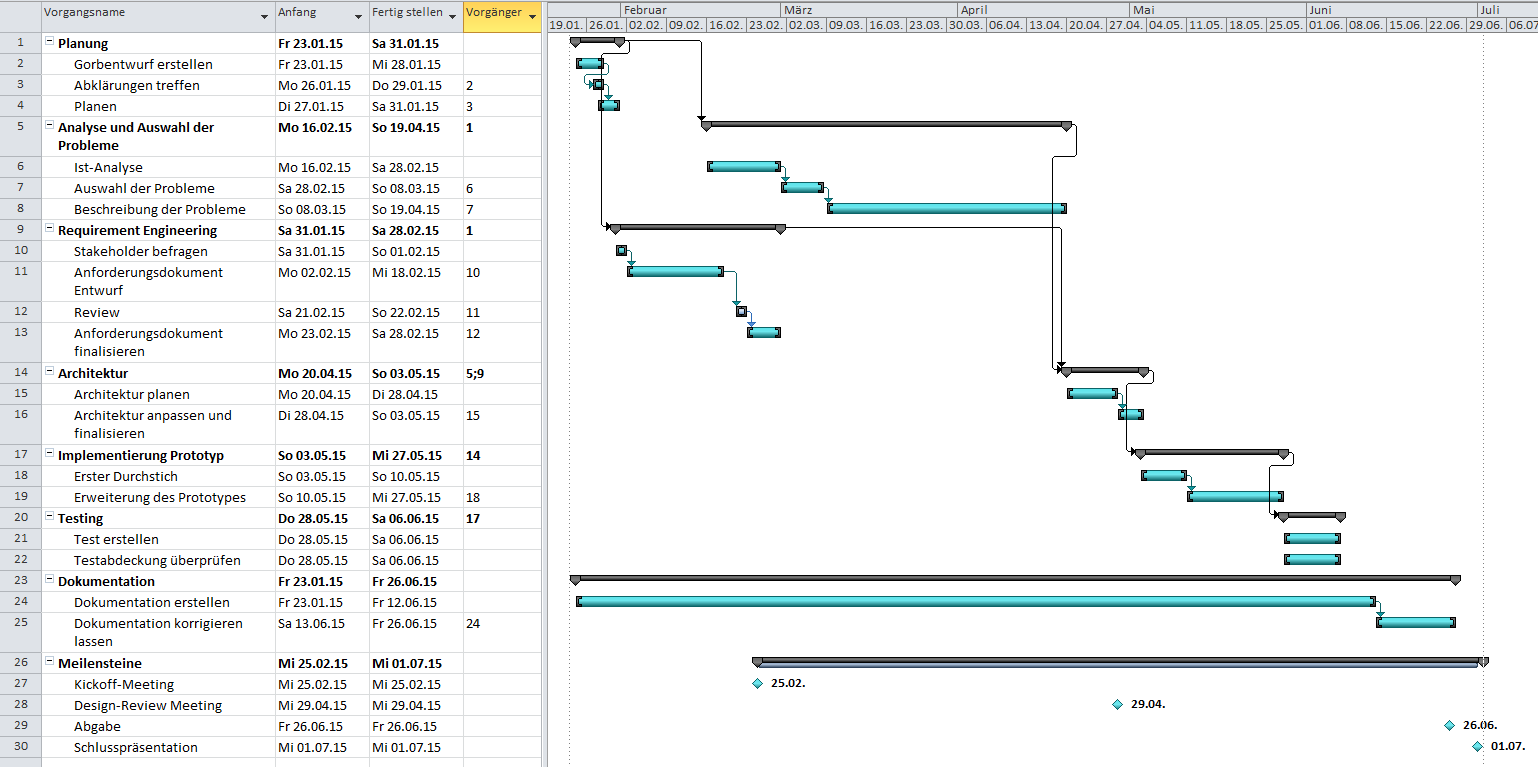
\includegraphics[scale=0.422]{images/project/projectplan.png}
\caption[Projektplan]{Projektplan \selfmade{}}
\label{fig:psp}
\end{figure}

\FloatBarrier

\subsection{Zeitschätzung auf Arbeitspaketebene}
\begin{table}[ht]
\centering
  \begin{tabular}{ l | c | c }
	\hline
	\rowcolor{gray}
	\textbf{Arbeitspaket}					&	\textbf{Schätzung (h)}	& \textbf{Tatsächlich (h)}	\\ \hline
	Requirement Engineering					&	20			& 30	\\ \hline
	Reale Optimierungsprobleme suchen			&	50			& 70	\\ \hline
	Wissensaufbau Algorithmen				&	70			& 50	\\ \hline
	Konzept Planung						&	60			& 70	\\ \hline
	Prototyp Entwicklung					&	50			& 80	\\ \hline
	Tests								&	10			& 20	\\ \hline
	Dokumentation						&	120			& 100	\\ \hline \hline
	Total								&	380			& 420	\\ \hline
  \end{tabular}
   \caption{Zeitschätzung auf Arbeitspaketebene}\label{table:time_estimation}
\end{table}

\FloatBarrier

\subsubsection{Erklärung der Abweichungen}
Das Requirement Engineering und Testen wurde unterschätzt, die Zeit floss jedoch vor allem in Detailarbeiten. Bei der Suche von realen Optimierungsprobleme wurde mehr Zeit beansprucht, als
ursprünglich geplant. Während der Suche konnte jedoch bereits Wissen über die Algorithmen aufgebaut werden, was dazu führte, dass in diesem Bereich weniger Zeit benötigt wurde. Als 
Evaluation des gewählten Konzept wurde ein \gls{vertikaler_durchstich} durchgeführt, was sich in der benötigten Zeit widerspiegelt. Die Entwicklung des Prototyps war aufwändiger 
als gedacht, was daran lag, dass sechs statt fünf Probleme umgesetzt wurden. Die Dokumentation benötigte nicht so viel Zeit, jedoch ist dieser Punkt auch etwas ungenau zu 
messen, da in den anderen Paketen bereits Dokumentation entsteht.
